\section{Components}

\subsection{Chip-Card}
We use simple memory cards with $I^2$C-Bus and form factor ID-00 as specifyed in ISO 7816. They are quite cheap (less then 1\euro{} per Card) and are not secure. Their contents might be easily read or modifyed. So everyone can read and check what we write on their card.

%-----

\subsection{realtimeclock (RTC)}
The realtimeclock is implemented in software by using one of the microcontrollers timers. A timerinterrupt function increments a 64bit value every millisecond (this counter will wrap arround in about 584.542.046 years, which should be quite enough for us). Additionaly the counters value is periodically\footnote{the value is backed up every $3FFFFF_{(16)}$ milliseconds wich is about every 1.165 hours} written to the microcontrollers eeprom and read back after reset. On reset we also add the value $3FFFFF_{(16)}$ to the counter to avoid having more then on time the same timestamp.

\subsection{random number generator (RNG)}
\begin{figure}
 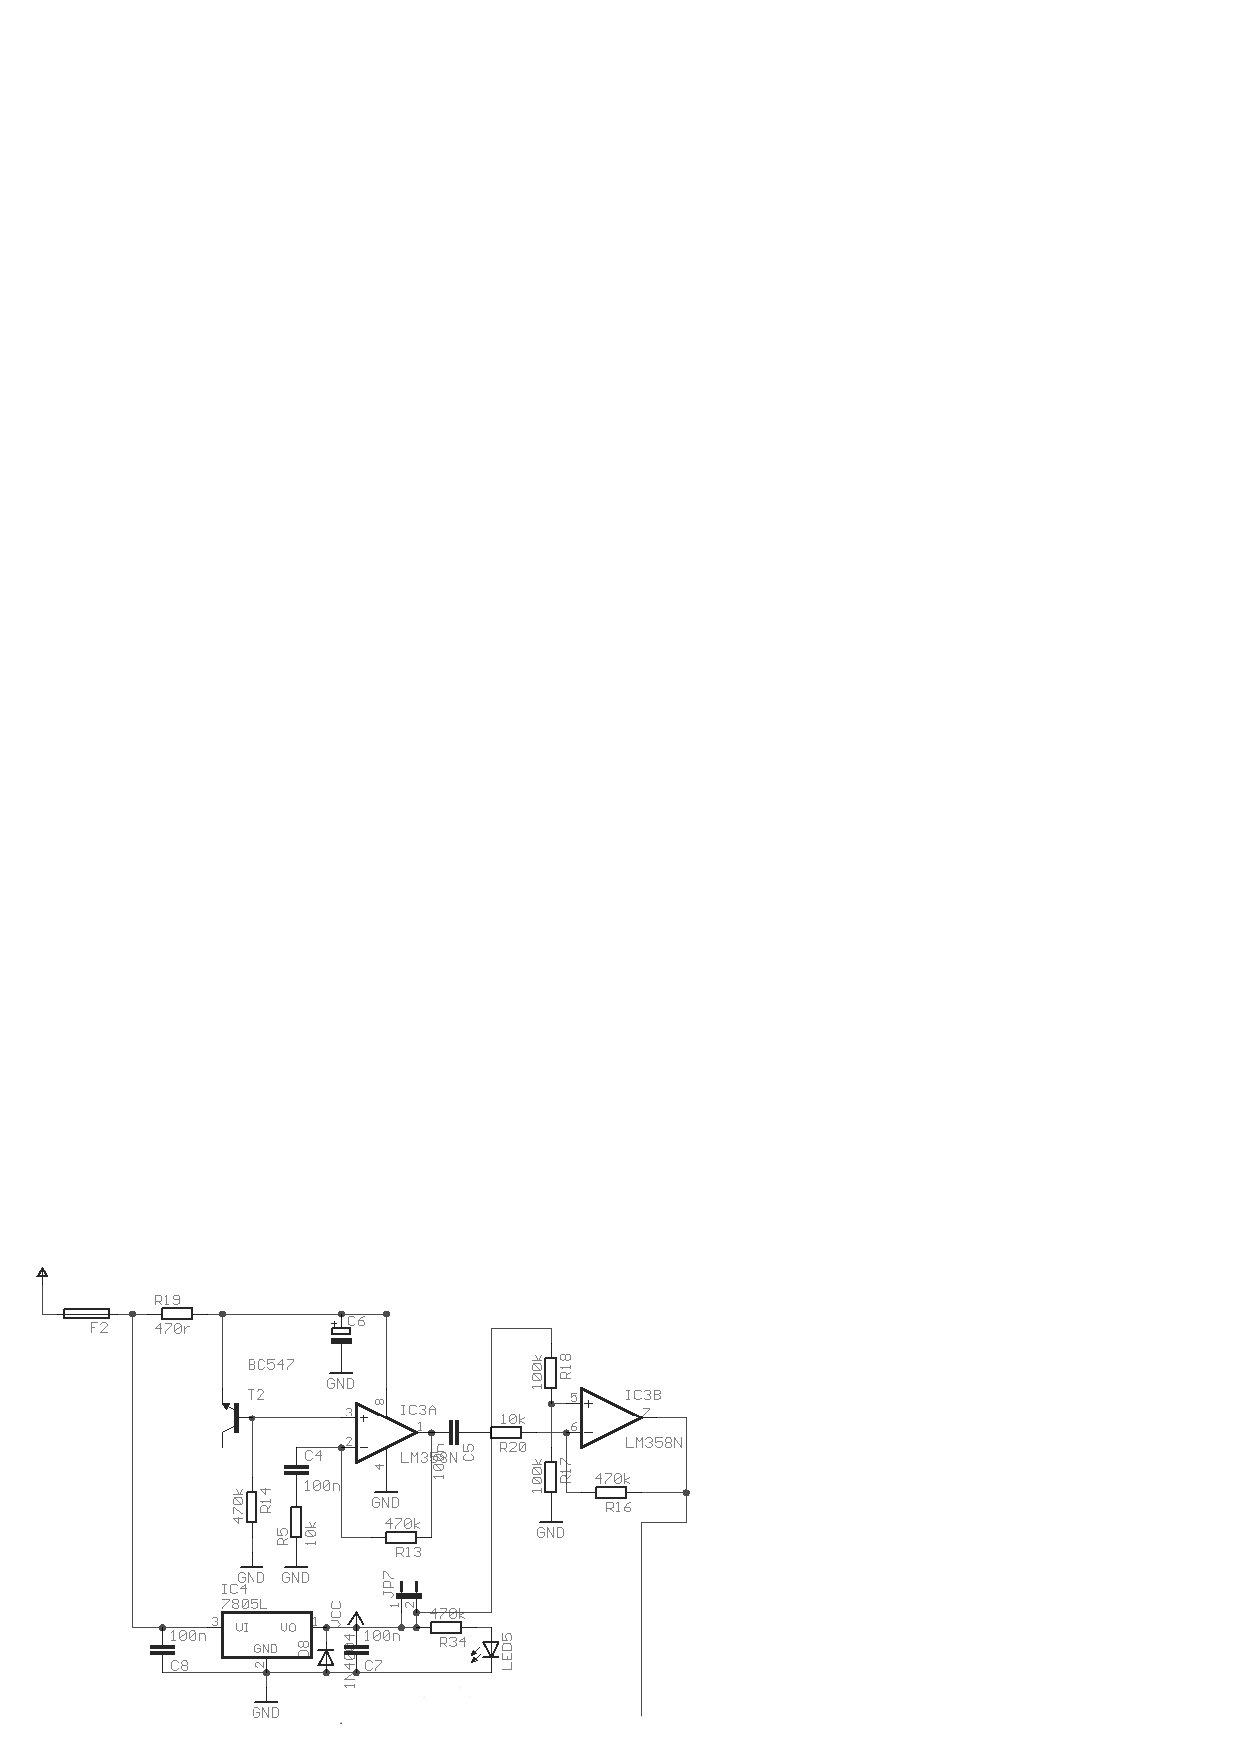
\includegraphics[scale=0.5]{RNG} 
\end{figure}

%-----

\subsection{pseudornadom number generator (PRNG)}

%-----

\subsection{secure serial port (QPort-tiny)}

%-----

\subsection{Ticket-Database (TicketDB)}

%-----

\subsection{FlackModifying-Database (FLMDB)}




